\documentclass{article}

% Language setting
% Replace `english' with e.g. `spanish' to change the document language
\usepackage[english]{babel}
\usepackage{enumitem}

% Set page size and margins
% Replace `letterpaper' with `a4paper' for UK/EU standard size
\usepackage[letterpaper,top=2cm,bottom=2cm,left=3cm,right=3cm,marginparwidth=1.75cm]{geometry}

% Useful packages
\usepackage{amsmath}
\usepackage{graphicx}
\usepackage{svg}
\usepackage{float}
% \usepackage{amsfonts}
\usepackage{multirow}
\usepackage[colorlinks=true, allcolors=blue]{hyperref}

% \title{ Mathematics in Machine Learning \\ \large Default of Credit Card Clients Dataset  Analysis}
% \author{Matteo Merlo \\ s287576}





\begin{titlepage}
\newgeometry{left=1cm,right=1cm,top=3cm,bottom=3.5cm}  %specific margins for this page

\begin{center}
\vspace{1cm}
{\large POLITECNICO DI TORINO}\\[1cm]
\textbf{\large Master’s Degree in Data Science and Engineering}\\[1.5cm]
%\textbf{Corso di Laurea Magistrale\\in Ingegneria Matematica}\\[3cm]
\includegraphics[width=0.45\textwidth]{logo_poli_blu.png}\\[1.5cm]

{\Large Mathematics in Machine Learning}\\[1cm]
%{\Large Tesi di Laurea Magistrale}\\[0.5cm]
\textbf{\Huge Default of credit card clients }\\[2cm]

\vspace{2cm}


\begin{minipage}{0.85\textwidth}
\begin{flushleft}\Large
\textbf{Professors} \hfill \textbf{Candidate}\\
prof. F. VACCARINO \hfill Matteo Merlo, 287576\\
prof. M. GASPARINI \\
\fillin\ \hfill \\
\fillin\ \hfill \fillin
\end{flushleft}
\end{minipage}

\vspace{1.5cm}
A.Y 2021-2022
\end{center}

\restoregeometry %restor default margins 

\end{titlepage}





\begin{document}
% \maketitle
% \begin{figure}
% \centering
% \includegraphics[width=0.8\textwidth]{logo_poli_blu.png}
% \end{figure}

\vspace{17cm}

\tableofcontents
\newpage

\begin{abstract}
The aim of this study is to exploit some supervised machine learning algorithms to identify the main factors that determine the probability of a credit card default, underlining the mathematical aspects and the methods used. Credit card defaults may occur when you have become severely broke on credit card payments. In order to increase market share, Taiwan's banks have issued excess cash and credit cards to unskilled applicants. At the same time, most cardholders, regardless of their repayment capability, were using their credit card excessively for consumption and have accumulated huge credits and debts.

The goal is to build an automated model to both identify central drivers and predict credit card default based on customer information and historical transactions. Next, the general concepts of the supervised machine learning paradigm are presented, along with a detailed explanation of all the techniques and algorithms used to build the models. In particular, Logistic Regression, Random Forest and Support Vector Machines algorithms have been applied.

The repository of this paper is available at: \href{https://github.com/MatteoM95/Default-of-Credit-Card-Clients-Dataset-Analisys}{https://github.com/MatteoM95/Default-of-Credit-Card-Clients-Dataset-Analisys}

\end{abstract}



\section{Introduction}

Since 1990, the Taiwanese government has allowed the formation of new banks. In order to increase market share, these banks have issued excess cash and credit cards to unskilled applicants. At the same time, most cardholders, regardless of their repayment ability, have abused their credit card for consumption and piled up heavy credit card debt and cash. Default occurs when a credit card holder is unable to comply with the legal obligation to repay. The crisis has caused a severe blow to confidence in consumer credit and has been a major challenge for both banks and cardholders \cite{uno}.

In a well-developed financial system, crisis management is downstream and risk prediction is upstream. The primary purpose of risk forecasting is to use financial information, such as corporate financial statements, customer transaction and refund records, etc., to predict individual customer business performance or credit risk and reduce damage and uncertainty.

In this project, the aim is to reliably predict who is at risk of defaulting. In this case, the bank may be able to prevent the loss by providing the customer with alternative options (such as forbearance or debt consolidation, etc.). Then, we build an automated model based on customer information and historical transactions that can identify key factors and predict credit card default.

\newpage
\section{Exploratory Data Analysis}

\subsection{Dataset Description}

The Default of Credit Card Clients dataset contains 30 000 instances of credit card status collected in Taiwan from April 2005 to September 2005. The dataset employs the binary variable \texttt{default payment next month} as response variable. It indicates if the credit card holders will be defaulters next month ($\text{Yes}=1, \text{No}=0$).
In particular, for each record (namely, each client) we have demographic information, credit data, history of payments and bill statements. To be more precise, the following is the complete list of all the 23 predictors \cite{due}.

\begin{itemize}
    \item Client personal information:
    \begin{enumerate}
        \item \texttt{LIMIT\_BAL}: Amount of given credit (in \textit{New Taiwan} dollars): it includes both the individual consumer credit and his/her family (supplementary) credit.
        \item \texttt{SEX} : 1 = male, 2 = female
        \item \texttt{EDUCATION}: 1 = graduate school; 2 = university; 3 = high school; 4 = others.
        \item \texttt{MARRIAGE}: Marital status, 1 = married; 2 = single; 3 = others.
        \item \texttt{AGE}: Age in years.
    \end{enumerate}
    \item History of past payments from April to September 2005, i.e., the delay of the past payment referred to a specific month:
    \begin{enumerate}[resume]
        \item \texttt{PAY\_0}: Repayment status in September, 2005.
        \item \texttt{PAY\_2}: Repayment status in August, 2005.
        \item \texttt{PAY\_3}: Repayment status in July, 2005.
        \item \texttt{PAY\_4}: Repayment status in June, 2005.
        \item \texttt{PAY\_5}: Repayment status in May, 2005.
        \item \texttt{PAY\_6}: Repayment status in April, 2005.
    \end{enumerate}
    The measurement scale for the repayment status is: -1 = pay duly; 1 = payment delay for one month; 2 = payment delay for two months; ...; 8 = payment delay for eight months; 9 = payment delay for nine months and above.
    \item Amount of bill statement (in \textit{New Taiwan} dollars), i.e. a monthly report that credit card companies issue to credit card holders in a specific month:
     \begin{enumerate}[resume]
        \item \texttt{BILL\_AMT1}: Amount of bill statement in September, 2005.
        \item \texttt{BILL\_AMT2}: Amount of bill statement in August, 2005.
        \item \texttt{BILL\_AMT3}: Amount of bill statement in July, 2005.
        \item \texttt{BILL\_AMT4}: Amount of bill statement in June, 2005.
        \item \texttt{BILL\_AMT5}: Amount of bill statement in May, 2005.
        \item \texttt{BILL\_AMT6}: Amount of bill statement in April, 2005.
     \end{enumerate}   
     \item Amount of previous payment (in \textit{New Taiwan} dollars):
     \begin{enumerate}[resume]
        \item \texttt{PAY\_AMT1}: Amount of previous payment in September, 2005.
        \item \texttt{PAY\_AMT2}: Amount of previous payment in August, 2005.
        \item \texttt{PAY\_AMT3}: Amount of previous payment in July, 2005.
        \item \texttt{PAY\_AMT4}: Amount of previous payment in June, 2005.
        \item \texttt{PAY\_AMT5}: Amount of previous payment in May, 2005.
        \item \texttt{PAY\_AMT6}: Amount of previous payment in April, 2005.

     \end{enumerate}  
\end{itemize}

In Figure 1 we can understand what the data looks like. The target \texttt{default.payment.next.month} is renamed \texttt{DEFAULT} to be short, while the PAY\_0 column is renamed PAY\_1

\begin{figure}[h]

\centering
\includegraphics[width=1\textwidth]{dfpandas.png}
\caption{Original dataset from UCI machine learning repository through pandas framework}
\end{figure}

\begin{table}[h]
\centering
\begin{tabular}{lllllll}
\# & Column     & Non-Null Count & Dtype &  &  &  \\ \cline{1-4}
0  & LIMIT\_BAL & 30000 non-null & int64 &  &  &  \\
1  & SEX        & 30000 non-null & int64 &  &  &  \\
2  & EDUCATION  & 30000 non-null & int64 &  &  &  \\
3  & MARRIAGE   & 30000 non-null & int64 &  &  &  \\
4  & AGE        & 30000 non-null & int64 &  &  &  \\
5  & PAY\_1     & 30000 non-null & int64 &  &  &  \\
6  & PAY\_2     & 30000 non-null & int64 &  &  &  \\
7  & PAY\_3     & 30000 non-null & int64 &  &  &  \\
8  & PAY\_4     & 30000 non-null & int64 &  &  &  \\
9  & PAY\_5     & 30000 non-null & int64 &  &  &  \\
10 & PAY\_6     & 30000 non-null & int64 &  &  &  \\
11 & BILL\_AMT1 & 30000 non-null & int64 &  &  &  \\
12 & BILL\_AMT2 & 30000 non-null & int64 &  &  &  \\
13 & BILL\_AMT3 & 30000 non-null & int64 &  &  &  \\
14 & BILL\_AMT4 & 30000 non-null & int64 &  &  &  \\
15 & BILL\_AMT5 & 30000 non-null & int64 &  &  &  \\
16 & BILL\_AMT6 & 30000 non-null & int64 &  &  &  \\
17 & PAY\_AMT1  & 30000 non-null & int64 &  &  &  \\
18 & PAY\_AMT2  & 30000 non-null & int64 &  &  &  \\
19 & PAY\_AMT3  & 30000 non-null & int64 &  &  &  \\
20 & PAY\_AMT4  & 30000 non-null & int64 &  &  &  \\
21 & PAY\_AMT5  & 30000 non-null & int64 &  &  &  \\
22 & PAY\_AMT6  & 30000 non-null & int64 &  &  &  \\
23 & DEFAULT    & 30000 non-null & int64 &  &  & 
\end{tabular}
\caption{Info returned by pandas on dataframe cointaining the given dataset}
\end{table}

\begin{table}[h]
\centering
\begin{tabular}{lllll}
\textbf{attribute}         & \textbf{value}  & \textbf{count} & \textbf{defaulters} & \textbf{(\%)} \\ \hline 
\multirow{2}{*}{SEX}       & Female          & 17.855         & 3.744               & 20,96\%       \\
                           & Male            & 11.746         & 2.861               & 24,35\%       \\ \hline 
\multirow{4}{*}{EDUCATION} & University      & 14.024         & 3.329               & 23,73\%       \\
                           & Graduate school & 10.581         & 2.036               & 19,24\%       \\
                           & High school     & 4.873          & 1.233               & 25,30\%       \\
                           & Other           & 123            & 7                   & 5,70\%        \\ \hline 
\multirow{3}{*}{MARRIAGE}  & Single          & 15.806         & 3.329               & 21,06\%       \\
                           & Married         & 13.477         & 3.192               & 23,68\%       \\
                           & Others          & 318            & 84                  & 26,4\%       
\end{tabular}
\caption{Value counts for \texttt{SEX}, \texttt{EDUCATION} and \texttt{MARRIAGE} feature}
\end{table}

\subsection{Data distribution}

From Figure 2 it is possible to see the distribution of the target variable \texttt{default\_payment\_next\_month}. It clearly shows an imbalance towards the 0 class (i.e. no default), with around 78\% of the whole dataset. This imbalance problem will make classification models focusing on the majority class overlooking the minority class if not addressed \cite{tre}.

\begin{figure}[H]
\centering
\includesvg[width=0.5\textwidth]{imbalanced_plot.svg}
\caption{Countplot of \texttt{default\_payment\_next\_month}}
\end{figure}

\subsection{Data Structure and cleaning} %from sofia perosin

So looking at the values present in the attributes some changes have to be done:
\begin{itemize}
    \item Attribute marriage should present only one of those values: 1,2,3; but in the dataset some records have value 0.
    \item Attribute education should present only one of those values: 1,2,3,4; but in the dataset some records have values 0,5,6.
    \item Attributes \texttt{PAY\_N} should present only one of those values: -1,1,2,3,4,5,6,7,8,9; but in the dataset some records have value -2 and 0.
\end{itemize}

In first two cases since there is an attribute which represent the \texttt{Other} class (respectively 3 for marriage and 4 for education), all the attributes not-known are mapped in that category. \newline
In the last case, in order to use this attributes as a numerical attribute, and not a categorical one, all the values -2 and -1 are mapped in 0. In this way \texttt{PAY\_N} will indicate for how many months the payment was delayed.


\subsection{Categorical features}
Regarding the categorical features \texttt{SEX}, \texttt{EDUCATION} and \texttt{MARRIAGE} showed in Figure 3 and counts in Table 2, it is possible to notice that there are much more females than males in the dataset, and, in particular, males have a slightly higher chance to default than females (0.24\% vs 0.21\%). But in general, whether it is male or female, the proportion of DEFAULTERS and NON-DEFAULTERS per each value, is in line with the categories of the other two features.

\begin{figure}[H]
\centering
\includesvg[width=1.1\textwidth]{categoricalDistribution.svg}
\caption{Countplot of \texttt{SEX}, \texttt{EDUCATION} and \texttt{MARRIAGE} grouped by DEFAULT class}
\end{figure}


We still have to inspect the payment status feature \texttt{PAY\_N}, boxplots below shown in Figure 4 is very useful. It can be seen that clients who delay payment by one month or less have fewer credit card defaults. I.e.  a greater discriminatory power is held the repayment status in September, \texttt{PAY\_1}, than the repayment status in the other months.

\begin{figure}[h]
\centering
\includesvg[width=1\textwidth]{BoxplotPAY.svg}
\caption{Boxplots of \texttt{PAY\_N} grouped by DEFAULT class}
\end{figure}


\subsection{Continuous features}
In statistics, the Kernel Density Estimation (KDE) is a fairly well known technique for estimating the probability density function in a non-parametric way (i.e. it does not assume any underlying distribution). So, for the following continuous feature, we explored their KDE plots.
Observing Figure 5 it is possible to notice that most of the default come from credits with a lower \texttt{LIMIT\_BAL} (i.e. credit amount), in particular they are observed in a range among a few thousands Taiwanese dollars to around \$140000. The customers above this threshold are more likely to repay their debts.

For the feature \texttt{AGE}, a similar visual analysis is performed. The probability of non-default of age between approximately 25 and 42 is higher, which indicates that consumers are more capable of repaying credit card loans in this age group. An assumption could be that their work and family tend to be stable without too much pressure.

\begin{figure}[H]
\centering
\includesvg[width=1\textwidth]{continuosDistribution.svg}
\caption{KDE plots of \texttt{LIMIT\_BAL} and \texttt{AGE} grouped by DEFAULT class}
\end{figure}

\subsection{Check for Normality distribution - QQ-plot}

Methods we will use later assume that the data should have a known and specific distribution, i.e. Normal distribution. Applying such methods on different data distribution, our final results may be misleading or plain wrong. A way to check whether our data are Normally distributed, we used a graphical method called Quantile-Quantile (QQ) plot that give us a qualitative evaluation. In a QQ-plot, the quantiles of the independent variable are plotted against the expected quantiles of the normal distribution. If the variable is normally distributed, the dots in the QQ-plot should fall along a 45 degree diagonal. The plots show that there is no evidence that numerical features are normally distributed.
\begin{figure}[h]
\centering
\includegraphics[width=1\textwidth]{QQplot.png}
\caption{QQ-plot for feature \texttt{LIMIT\_BAL}, \texttt{BILL\_ATM},\texttt{AGE} and \texttt{PAY\_ATM}}
\end{figure}


\subsection{Correlation} % di salvo
Correlation is a statistical term describing the degree to which two random variables move in coordination with one-another. Intuitively, if they are moving in the same direction, then those variables are defined with a positive correlation, or viceversa we define that with a negative correlation. The Pearson Correlation ($\rho$) is one
of the most used linear correlation measures.

\begin{equation}
\rho(X, Y ) =\frac{Cov(X, Y)}{\sigma_{X} \sigma_{Y}} = \frac{E[(X-\mu_{X})(Y-\mu_{Y})]}{\sigma_{X} \sigma_{Y}}
\end{equation}

The value of Pearson’s Correlation Coefficient range is $[$ -1, 1 $]$.
\begin{itemize}
    \item +1 means that they are strongly correlated.
    \item 0 means no correlation, the two random variables are statistically independent, but it is not true the opposite, because they may have a non-linear relationship.
    \item -1 means that there is a negative correlation (inverse proportion).
\end{itemize} 

High values of this correlation coefficient with respect to the target is a synonym of data redundancy, so it could be helpful to drop those columns. In Figure 7 is given a graphical representation of the Person Correlation with a Heatmap, where each cell $(i, j)$ represents the Person Correlation between the random variables $X_{i}$ and $X_{j}$

From Figure 7, as we may think, we can observe an "internal" correlation among the groups of features such as \texttt{BILL\_ATM}, \texttt{PAY\_N}. We can also notice that there is no feature with a strong relationship with the target. In fact, there are 15 features with an absolute value of the correlation below than 0.1 and none of the remaining ones have a greater correlation than 0.29.

\begin{figure}[H]
\centering
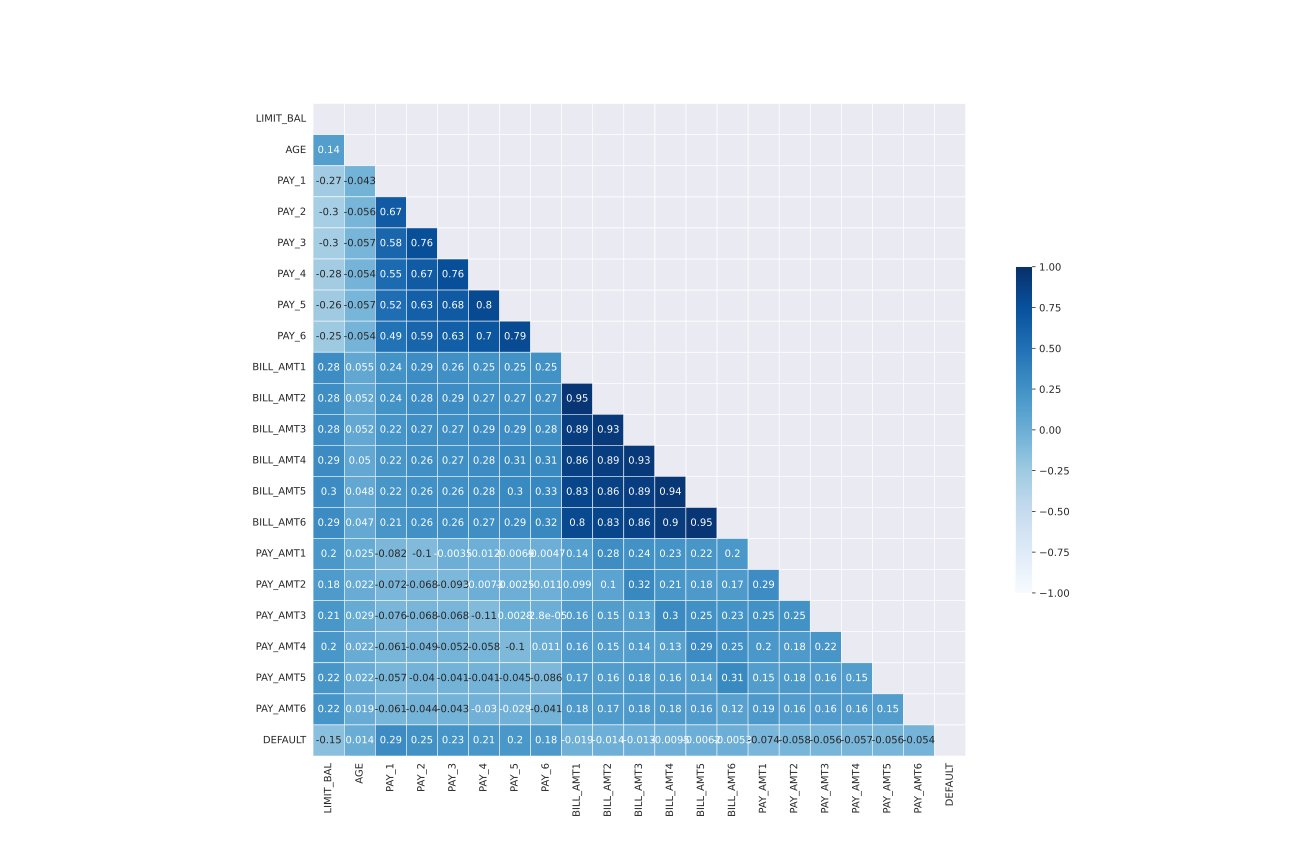
\includegraphics[width=1.1\textwidth]{correlation.png}
\caption{Heatmap correlation}
\end{figure}


%%%%%%%%%%%%%%%%%%%%%%%%%%%%%%%%%%%%%%%%%%%%%%%%%%%%%%%%%%%%%%%%%%%%%%%%%%%55
\newpage
\section{Data preprocessing}
\subsection{Handling Categorical Features}
The categorical features \texttt{EDUCATION}, \texttt{SEX}, and \texttt{MARRIAGE} are already encoded with integer numbers and could be fed to a machine learning algorithm. However, these are nominal features, for which it would be sub-optimal to assume an ordering. \emph{One-hot encoding} allows us to remove any ordinal relationship, which would be meaningless between these categorical variables. The idea behind this approach is to create a new dummy feature for each unique value in the nominal feature column. Binary values can then be used to indicate the particular class of an example.

Although Scikit-Learn provides methods to perform one-hot encoding automatically, we decide to do the mapping of the features by hand, since there are few. In this way we mitigate the problem of \emph{multicollinearity}, which occurs when there are highly correlated features. Thus, we create the following boolean columns and drop the old ones, \texttt{EDUCATION}, \texttt{SEX}, and \texttt{MARRIAGE}.

\begin{itemize}
    \item \texttt{MALE}: 1 = male; 0 = female.
    \item \texttt{MARRIED}: 1 = married marital status; 0 = otherwise.
    \item \texttt{GRAD\_SCHOOL}: 1 = graduate school level of education; 0 = otherwise.
    \item \texttt{UNIVERSITY}: 1 = university level of education; 0 = otherwise.
    \item \texttt{HIGH\_SCHOOL}: 1 = high school level of education; 0 = otherwise.
\end{itemize}

Using this strategy we do not loose any information.
In Table 3 and Table 4 there is an example that shows variable respectively before and after the application of one-hot encoding.

\begin{table}[H]
\centering
\begin{tabular}{llll}
\textbf{id} & \textbf{\texttt{SEX}} & \textbf{\texttt{MARRIAGE}} & \textbf{\texttt{EDUCATION}} \\ \hline
0           & 1            & 1                 & 1                  \\
1           & 2            & 2                 & 2                  \\
2           & 1            & 3                 & 3                  \\
3           & 2            & 1                 & 4                 
\end{tabular}
\caption{\texttt{SEX}, \texttt{MARRIAGE} and \texttt{EDUCATION} features before one-hot encoding}
\end{table}

\begin{table}[H]
\centering
\begin{tabular}{lllllll}
\textbf{id} & \textbf{\texttt{MALE}} & \textbf{\texttt{MARRIED}} & \textbf{\texttt{SINGLE}} & \textbf{\texttt{GRAD\_SCHOOL}} & \textbf{\texttt{UNIVERSITY}} & \textbf{\texttt{HIGH\_SCHOOL}} \\ \hline
0           & True          & True             & False           & True                  & False               & False                 \\
1           & False         & False            & True            & False                 & True                & False                 \\
2           & True          & False            & False           & False                 & False               & True                  \\
3           & False         & True             & False           & False                 & False               & False                
\end{tabular}
\caption{\texttt{SEX}, \texttt{MARRIAGE} and \texttt{EDUCATION} features after one-hot encoding}
\end{table}

\subsection{Dataset Partition}

A common practice, in order to evaluate the performances of a classification algorithm, is to divide the dataset into two partitions, called training and test set. The training set is used to fit the machine learning model, whereas the test set is used to evaluate the fit machine learning model. In this case, since there is
a adequate number of samples, 75\% of the initial dataset is used for the training procedure and the remaining 25\% for testing, while preserving the initial data distribution (attribute \emph{stratify}).

Another data splitting is necessary, in order to tune the hyperparameters. In particular, two new partitions will be considered: train set and validation set. It has been used a Stratified K-Fold Cross Validation (with k = 5). Once obtained the best hyperparameters, train again the model with both train and evaluation set and finally evaluate it on the test set.

\begin{itemize}
    \item Training set:
    \begin{itemize}
        \item shape: (22200,25)
        \item defaulters: 4955
        \item non-defaulters: 17245
        \item class proportion: 22,30\%
    \end{itemize}
    \item Test set:
     \begin{itemize}
        \item shape: (7400,25)
        \item defaulters: 1650
        \item non-defaulters: 5750
        \item class proportion: 22,30\%
    \end{itemize}
\end{itemize}

% \begin{figure}[h]
% \centering
% \includegraphics[width=0.6\textwidth]{datasetsplitting.png}
% \caption{Dataset Splitting}
% \end{figure}
%%%%%%%%%%%%%%%%%%%%%%%%%%%%%%%%%%%%%%%%%%%%%%%%%%%%%%%%%%%%%%%%%%%%%%%%%%%%%%%%%%%%555
\subsection{Outliers and Anomaly detection}
An outlier or an anomaly detection is an observation that deviates so much from other observations as to arouse suspicion that it was generated by a different mechanism. Some of the most common causes of outliers are:
\begin{itemize}
    \item an entity may seem different because it belongs to another class;
    \item  there is always the probability (even if it is lower) that we record real values far from the regular patterns;
    \item some technical or human errors occur.
\end{itemize}

The presence of a significant amount of outliers in some cases could drastically affect the performances. Therefore, it is a common practice to train the model with and without them in order to catch their contribution. 
There are several different techniques for removing outliers. It is possible to find them thanks to some graphical representation of the data (e.g. Boxplot).

Figure 8 shows the boxplots for \texttt{BILL\_ATM} and  \texttt{PAY\_ATM} variables, and are each followed by a description of how outliers were determined for the variables.
The \texttt{BILL\_ATM} variables were depicted the amount of bill statement during the respective months. Since these can actually be considered as repeated observations of the same variable (per cardholder), then for the purpose of outlier identification, they were analyzed using the same boxplot. In addition, and to minimize the loss of information due to elimination of outliers, a cut-off value was set for these variables based on the general trend observed in the six variables. Consequently, it was assumed that for all \texttt{BILL\_ATM} variables, any amount exceeding 1,000,000 and any amount going below $min(\texttt{BILL\_ATM4})$, which was the value 170,000, was considered to be an outlier.

For the \texttt{PAY\_ATM} variables, the same approach was takes for outlier detection as the one taken for \texttt{BILL\_ATM} variables. The general trend of the six variables set the upper cut-off point at $max(\texttt{PAY\_ATM4})$ which was the value 621,000. Any observation exceeding this amount was considered an outlier. On the lower side, no observation had a value lower than 0, hence there were no outliers based on this (taking 0 as the minimum).
After the exclusion of outlier values was done, a sample size of 29,993 remained (7 observations were dropped), which was the data used for training and validating the model \cite{ventidue}.

We do not eliminate any sample as an outlier because the literature on the dataset does not provide information on this \cite{diciasette}, and we lack knowledge about the domain.

\begin{figure}[h]
\centering
\includegraphics[width=1\textwidth]{outliers.png}
\caption{Box-plot for \texttt{PAY\_ATM} and \texttt{BILL\_ATM} Variables}
\end{figure}

\subsection{Features Scaling}

The majority of machine learning and optimization algorithms behave much better if numerical features are on the same scale. Decision trees and random forests are two of the very few machine learning algorithms where there is no need to worry about feature scaling, as they are scale invariant \cite{quattro}.

There are two common approaches to bringing different features onto the same scale: 
\begin{itemize}
    \item \emph{Normalization} refers to the rescaling of the features to a range of [0, 1], in this case we use min-max scaling:
    \begin{equation}
    X_{Norm} = \frac{X - X_{Min}}{X_{Max} - X_{Min}}
    \end{equation}
    where $X$ is a particular example, $X_{Min}$ is the smallest value in a feature column, and $X_{Max}$ is the largest value.
    
    \item \emph{Standardization or Z-Score Normalization}: center the feature columns at mean $\mu$ = 0,  with standard deviation $\sigma = 1$, so that the feature columns have the same parameters as a standard normal distribution, which makes it easier to learn the weights: 
    \begin{equation}
    Z = \frac{X - \mu }{\sigma }
    \end{equation}
\end{itemize}

While normalization suppress the effect of outliers, standardization maintains information about them. Since the technique we will apply shortly is sensitive to the presence of outliers, we decide to continue our study with the normalized data.

\begin{figure}[h]
\centering
\includegraphics[width=1\textwidth]{scalingfeature.png}
\caption{Box-plot scaled features}
\end{figure}

\subsection{Dimensionality reduction}

As we mentioned previously, many algorithms would benefit from the removal of strongly correlated features, and in general from having a lower dimensionality of the data. The presence of many features in the dataset leads to excessively complex models, which fit the parameters too closely with regard to the particular observations in the training set, but do not generalize well to new data. We say that these models have a high variance and are overfitting the training set.

In fact, high dimensional data can overfit the training set. The problem of overfitting become more serious i.e. in Nearest Neighbor classifiers, where the course of dimensionality problem is faced. The curse of dimensionality depicts the phenomenon where the feature space becomes progressively sparse for an increasing number of dimensions of a fixed-size training dataset. We can think of even the nearest neighbors as being excessively far away in a high-dimensional space to give a good estimate.

The dimensionality reduction can be carried out by means of:

\begin{itemize}
    \item \emph{feature selection}: we select a subset of the original features
    \item \emph{feature extraction}: we construct a new feature subspace deriving information from the original feature set.
\end{itemize}

As previously noticed, \texttt{BILL\_ATM} categories are highly correlated between them, so a manual discard could be done. However, we decide to keep them to perform \emph{Principal Component Analysis}, a feature extraction technique.

\subsubsection{PCA - Principal component analysis}

In PCA, both the compression and the recovery, are performed by linear transformations. Let $x_{1}, ... x_{m}$, be $m$ vectors in $ \mathbb{R_{d}}$. We would like to reduce the dimensionality of these vectors using a linear transformation.

The idea is to find a matrix $W \in \mathbb{R^{n,d}}$, where $n < d$, that induces a mapping

\begin{equation}
x \mapsto \mathbb{W_{x}}, ~~~ x \in \mathbb{R^{d}}, W_{x} \in \mathbb{R^{n}};  ~~~ (n<d)
\end{equation}

and a second matrix $U \in \mathbb{R^{n,d}}$, that can be used to recover each original vector $x$ from its compressed version. That is, for a compressed vector $y = \mathbb{W}x$, where $y$ is in the low dimensional space $\mathbb{R^{n}}$, we can construct $\Tilde{x}=\mathbb{U}y$, so that $\Tilde{x}$ is the recovered version of $x$ and resides in the original high dimensional space $\mathbb{R^{d}}$.

The objective of PCA is to find the compression matrix $\mathbb{W}$ and the recovering matrix $\mathbb{U}$ so that the total squared distance between original and recovered vector is minimal in the least squared sense:

\begin{equation}
\underset{\mathbb{W}\in\mathbb{R^{n,d}},\mathbb{U}\in\mathbb{R^{d,n}}}{argmin} \sum_{i=1}^{m} \left \| \textbf{x}_{i}-\mathbb{UW}\textbf{x}_{i}  \right \|_{2}^{2}
\end{equation}

The optimal solution ($\mathbb{U}$, $\mathbb{W}$) of this problem takes the form:

\begin{itemize}
    \item the columns of $\mathbb{U}$ are orthonormal: $\mathbb{U}^{\top}\mathbb{U} = \mathbb{I}_{n}\in \mathbb{R}$;
    \item $\mathbb{W} = \mathbb{W^{\top}}$
\end{itemize}

Hence, we can write:

\begin{equation}
\underset{\mathbb{U}\in\mathbb{R^{d,n}}: \mathbb{U}^{\top}\mathbb{U}=\mathbb{I}_{n} }{argmin} \sum_{i=1}^{m} \left \| \textbf{x}_{i}-\mathbb{U}^{\top}\mathbb{U}\textbf{x}_{i}  \right \|_{2}^{2}
\end{equation}

It can be proven that:

\begin{equation}
\left \| \textbf{x}-\mathbb{U}^{\top}\mathbb{U}\textbf{x}  \right \|^{2} = \left \|  \textbf{x} \right \|^{2} - tr(\mathbb{U}^{\top}\textbf{x}\textbf{x}^{\top}\mathbb{U})
\end{equation}

where the trace \emph{tr}  of a matrix is the sum of its diagonal entries, i.e., a linear operator. This allows us to rewrite Equation (6) as the following maximization problem:

\begin{equation}
\underset{\mathbb{U}\in\mathbb{R^{d,n}}: \mathbb{U}^{\top}\mathbb{U}=\mathbb{I}_{n} } {argmax} tr(\mathbb{U}^{\top} (\sum_{i=1}^{m} \textbf{x}_{i}\textbf{x}^{\top}) \mathbb{U})
\end{equation}

Now, we can define the scatter matrix $ \mathbb{A} = \sum_{i=0}^{m} x_{i}x_{i}^{\top}$, since this matrix is symmetric, it can be written using its spectral decomposition $ \mathbb{A} =  \mathbb{VDV^{\top}} $, where  
$\mathbb{D}$ is diagonal and $ \mathbb{V^{\top}}\mathbb{V} = \mathbb{V}\mathbb{V^{\top}} = \mathbb{I}$. Here, the elements on the diagonal of  
$\mathbb{D}$ are the eigenvalues of $\mathbb{A}$, while the columns of $\mathbb{V}$ are the corresponding eigenvectors. In particular, we can safely assume that the diagonal elements of 
$\mathbb{D}$ are sorted by the largest, and are all positive because $\mathbb{A}$ is semi-definite positive:

\begin{equation}
\mathbb{D_{1,1}} \geq \mathbb{D_{2,2}} \geq ... \geq \mathbb{D_{d,d}} \geq 0
\end{equation}

From these premises, we can claim that the solution of the optimization problem (6) is the matrix $\mathbb{U}$, whose columns $\textbf{u}_{1}, ...., \textbf{u}_{n} $ are the \emph{n} eigenvectors of the matrix $\mathbb{A}$ corresponding to the largest \emph{n} eigenvalues, while $\mathbb{W} = \mathbb{U^{\top}} $.

So to sum up, PCA helps us to identify patterns in the data based on the correlation between features, finding the directions of maximum variance in high-dimensional data and projecting it onto a new subspace with equal or fewer dimensions than the original one.

The orthogonal axes (PC = principal components) of the new subspace can be interpreted as the directions of maximum variance given the constraint that the new feature axes are orthogonal to each other, as illustrated in the Figure 10. Here, $x_{1}$ and  $x_{2}$ are the original feature axes, and $PC_{1}$ and $PC_{2}$ are the principal components \cite{cinque}.

\begin{figure}[h]
\centering
\includegraphics[width=0.6\textwidth]{PCA2D.png}
\caption{PCA graphical explanation}
\end{figure}

Since a reduction of the dimensionality of our dataset can be done by compressing it onto a new feature subspace, the number of principal components chosen will be that preserve at the most the information carried by the data. A decision can be taken looking at the explained variance ratio, that will be how much variance does contain each principal component out of the \emph{d} components we obtain applying PCA to our training dataset.

Results depicted in Figure 11 show that the first 6 principal components capture more than 90\% of the total variance. However, considering the first 12 principal components the variance is capable to explain 99\% of the total variance, even if the number of features is halved.

\begin{figure}[H]
\centering
\includesvg[width=0.7\textwidth]{PCACumulative.svg}
\caption{Cumulative and individual explained variance plotted against principal components}
\end{figure}


\subsection{Class imbalance - Resampling}

Class imbalance is quite a common problem when working with real-world data, it consists of having much more samples that refers to one class than other classes in the dataset.
We showed in Section 2.2 and reported in Figure 2 that the dataset we are dealing with is unbalanced, as the non-defaulter examples are over-represented.

In our case, we could achieve almost 80\% accuracy by just predicting the majority class (non-defaulters) for all examples, without the help of a supervised machine learning algorithm. Thus, when we will fit classifiers on our datasets, it would make sense to focus on other metrics than accuracy when comparing different models.

Aside from evaluating machine learning models, class imbalance influences a learning algorithm to model fitting itself. Since machine learning algorithms typically optimize cost function that is computed as a sum over the training examples that it sees during fitting. The decision rule is likely going to be biased toward the majority class.

The option of collecting more data is excluded a priori. There are other option to tackle this problem:
\begin{itemize}
    \item At training time assign larger penalty to wrong predictions on the minority class. 
    \item Upsampling the minority class
    \item Downsampling the majority class
\end{itemize}

Unfortunately, there is not a generalized best solution or technique that works best across different problem domains. Thus, in practice, it is recommended to try out different strategies on a given problem, evaluate the results, and choose the technique that seems most appropriate.

We decide to exclude the naïve methods of oversampling (undersampling), since they randomly duplicate (delete) data from the minority (majority) class, until the desired level is obtained. On the one hand, random undersampling does not allow controlling which information is discarded, on the other hand random oversampling causes overfitting because the model is trained on many identical data. We decide to explore two technique which mitigate exposed issues that are the Cluster Centroid (Undersampling) method and the Synthetic Minority Oversampling Technique (SMOTE).

\begin{figure}[H]
\centering
\includegraphics[width=0.6\textwidth]{resampling.png}
\caption{Resampling techniques}
\end{figure}

\subsubsection{Cluster Centroid Undersampling}

Minority class samples in our dataset are enough to allow us to perform undersampling. However, one major problem of using undersampling is that important information may be lost from the majority class, which can cause overly general rules. This cannot be afforded to develop the credit card default prediction model, especially for default samples. Hence, to overcome this problem, the Cluster Centroids method has been introduced in \cite{sei}.

The idea of the Cluster Centroids method is to replace clusters of majority samples with the respective cluster centroids. A K-means algorithm is fitted to the data, and the number of clusters is set equal to the number of samples of the minority class. Then, the majority of samples from the clusters are entirely substituted by the sets of cluster centroids from K-means \cite{sette}. Cluster Centroids contain the most representative variations of the majority class in which features values would be visualized at the center.

\begin{figure}[h]
\centering
\includegraphics[width=0.45\textwidth]{clusterundersampling.png}
\caption{Cluster centroids undersampling \cite{otto}}
\end{figure}

\subsubsection{SMOTE - Synthetic Minority Oversampling Technique}

The Synthetic Minority Oversampling Technique (SMOTE) was proposed in \cite{nove} to avoid the risk of overfitting faced by random oversampling. Instead of simply replicating existing observations, the technique generates artificial samples. As shown in Figure 14, this is achieved by linearly interpolating a randomly selected minority observation and one of its neighboring minority observations. More precisely, SMOTE executes three steps to generate a synthetic sample:

\begin{itemize}
   \item Firstly, it chooses a random minority observation $\vec{a}$
   \item Among the nearest minority of $\vec{a}$ neighbors select the instance $\vec{b}$
   \item Create a new sample $\vec{x}$ by linearly interpolating $\vec{a}$ and $\vec{b}$ (with $\omega$ random)
   
   \begin{equation}
   \vec{x} = \vec{a} + \omega \times (\vec{b} - \vec{a}), ~~~ \omega \in [0,1]
   \end{equation}
\end{itemize}

\begin{figure}[H]
\centering
\includegraphics[width=1\textwidth]{smote.png}
\caption{SMOTE linearly interpolates a randomly selected minority sample and one of its k = 4 nearest neighbors \cite{dieci}}
\end{figure}

Unfortunately, SMOTE, as other random oversampling techniques, suffers from weakness due to within-class imbalance and noise. In fact, SMOTE choose a random sample from the minority class to start, but if distribution of the minority class is not uniformed this can cause densely populated areas to be further inflated with artificial data. Moreover, SMOTE does not recognize noisy minority samples which are located among majority class instances and interpolate them with their minority neighboring, may be creating new noisy entries.

Finally, it has been proven that classification algorithms could benefit from samples that are closer to class boundaries, and SMOTE does not specifically work in this sense, as shown in Figure 15.

\begin{figure}[H]
\centering
\includegraphics[width=0.7\textwidth]{smotebehaviour.png}
\caption{SMOTE behavior in presence of noise and with-in class imbalance \cite{dieci}}
\end{figure}

\subsubsection{K-means SMOTE}

As showed in \cite{dieci} the method employs the simpler and popular K-means clustering algorithm in conjunction with SMOTE oversampling in order to rebalance datasets. It manages to avoid the generation of noise by oversampling only in safe areas (i.e., areas made up of at least 50\% of minority samples). Moreover, its focus is placed on both between-class imbalance and within-class imbalance, fighting the small disjuncts' problem by inflating sparse minority areas.
K-means SMOTE executes three steps as show in Figure 16: clustering, filtering, and oversampling.

\begin{itemize}
    \item Clustering: the input space is clustered into k groups using K-means clustering. 
    \item Filtering: selects clusters for oversampling, retaining those with a high proportion of minority class samples. It then distributes the number of synthetic samples to generate, assigning more samples to clusters where minority samples are sparsely distributed. 
    \item Oversampling: SMOTE is applied in each selected cluster to achieve the target ratio of minority and majority instances.
\end{itemize}



\begin{figure}[H]
\centering
\includegraphics[width=0.7\textwidth]{KMeansSMOTE.png}
\caption{K-means SMOTE over samples safe areas and combats within-class imbalance }
\end{figure}


%%%%%%%%%%%%%%%%%%%%%%%%%%%%%%%%%%%%%%%%%%%%%%%%%%%%%%%%%%%%%%%%%%%%%%%%%%%%%%5
\newpage
\section{Model evaluation}

One of the main steps in building a machine learning model is to estimate its performance on data that the model has not seen before. For this reason, in 3.2 initial dataset is splitted into separate training and test datasets. The former will be used for model training, and the latter to estimate its generalization performance. This approach is commonly known as holdout method.

However, in typical machine learning applications, it is interested in tuning and comparing different parameter settings to further improve the performance for making predictions on unseen data. But, if we reuse the same test dataset over and over again during this process, it will become part of our training data and thus the model will be more likely to overfit. A validation set could be held out of the training set, to evaluate on it the performance of the model. However, this is not recommended because performance estimation may be sensitive to how we partition the training set. 

\subsection{K-fold cross validation}
%maggio
Instead of holdout, a more robust technique for model tuning is k-fold cross-validation, where we repeat the holdout method \emph{k} times on \emph{k} subsets of the training data. 
In practice, we randomly split the training dataset into \emph{k} folds without replacement, where \emph{k-1} folds are used for the model training, and one fold is used for performance evaluation. We then calculate the average performance of the models based on the different independent test folds to obtain a performance estimate that is less sensitive to the sub-partitioning of the training data compared to the holdout method. Once we have found satisfactory hyperparameter values, we can retrain the model on the complete training dataset and obtain a final performance estimate using the independent test dataset.
The rationale behind fitting a model to the whole training dataset after k-fold cross-validation is that providing more training examples to a learning algorithm usually results in a more accurate and robust model.

\begin{figure}[h]
\centering
\includegraphics[width=0.5\textwidth]{kfold.png}
\caption{K-fold cross validation }
\end{figure}
%antonio
Since k-fold cross validation is a resampling technique without replacement, its advantage is that each sample of the training set will be used exactly once for validation purpose, and this yields to a lower-variance estimate of the model performances than the holdout method.
A common value for \emph{k} in k-fold cross validation is 10 \cite{undici}. However, we are dealing with a large dataset and choosing such a value would be too costly in computational sense, for this reason we decide to use a smaller value for \emph{k}, i.e. \emph{k} = 5, still taking advantage of the k-fold method.

\subsection{Performance evaluation metrics}
Classification evaluation metrics compare the predicted class from the classifier with the actual class of the samples. At this scope it is useful to build a confusion matrix where the \emph{(j, k)-th} element counts the number of times that the actual class is \emph{j} whereas the predicted class is \emph{k}.
In the binary case (such as our case) the confusion matrix become simpler to build and to
interpret. If the two classes to be predicted are True and False the confusion matrix is the one depicted in Table 5.

\begin{table}[H]
    \centering
   \begin{tabular}{ll|ll}
                                 &          & \multicolumn{2}{l}{Actual Class} \\
                                 &          & Positive        & Negative       \\ \hline
\multirow{2}{*}{Predicted Class} & Positive & TP              & FP             \\
                                 & Negative & FN              & TN            
    \end{tabular}
    \caption{Binary classification confusion matrix}
    \label{tab:my_label}
\end{table}

The following terminology is used when referring to the counts tabulated in a confusion matrix:

\begin{itemize}
    \item \emph{True positive (TP)}, which corresponds to the number of positive examples correctly predicted by the classification model.
    \item \emph{False negative (FN)}, which corresponds to the number of positive examples wrongly predicted as negative by the classification model.
    \item \emph{False positive (FP)}, which corresponds to the number of negative examples wrongly predicted as positive by the classification model.
    \item \emph{True negative (TN)}, which corresponds to the number of negative examples correctly predicted by the classification model. 
\end{itemize}

\begin{figure}[h]
\centering
\includegraphics[width=1\textwidth]{precisionrecall.png}
\caption{Precision and Recall}
\end{figure}

Different metrics can be used depending on the task, the data imbalance and other factors. While dealing with classification tasks, these are some of the most used ones:

\begin{itemize}
    \item \emph{Accuracy}: is the performance measure generally associated with machine learning algorithms. It is the ratio of correct predictions over the total number of data points classified. 
    \begin{equation}
    Accuracy = \frac{TP + TN}{TP + FP + TN + FN}
    \end{equation}
    
    \item \emph{Precision}: (also called \emph{positive predictive} value): Indicates how many of a \emph{j}-object (in binary classification, commonly True class is considered) predictions are correct. It is defined as the ratio of correct positive predictions over all the positive predictions.
    \begin{equation}
    Precision = \frac{TP}{TP + FP}
    \end{equation}
    
    \item \emph{Recall}: (also called \emph{sensitivity}): Indicates how many of the \emph{j}-object (in binary classification, commonly True class is considered) samples are correctly classified. It is defined as the fraction of j-object predictions over the total number of \emph{j}-object samples.
    
    \begin{equation}
    Recall = \frac{TP}{TP + FN}
    \end{equation}
    
    \item \emph{F1}: Accuracy measure treats every class as equally important, for this reason it may be not suitable for imbalanced datasets, where the rare class is considered more interesting than the majority class \cite{dodici}. 
    
    Hence, Precision and Recall, that are class-specific metrics, are widely employed in applications in which successful detection of the rare class is more significant than detection of the other.
    
    The challenge is to build a model that is capable of maximize both Precision and Recall. Hence, the two metrics are usually summarized in a new metric that is F1-score. In practice, F1-score represents the harmonic mean between precision and recall, so, a high value ensures that both are reasonably high.
    \begin{equation}
    F1_{score} = \frac{2}{\frac{1}{r}+\frac{1}{p}} = \frac{2rp}{r + p}, ~~~~ where ~ r=Recall, p=Precision
    \end{equation}
\end{itemize}

%%%%%%%%%%%%%%%%%%%%%%%%%%%%%%%%%%%%%%%%%%%%%%%%%%%%%%%%%%%%%%%%%%%%%%%%%%%%%%%%%%%%%%%
\newpage
\section{Classification models}
In this section, we present different supervised learning algorithms with their mathematical details, and we use them on our dataset to build a classification model that is able to predict credit card defaults in the next month. In particular we will dive into Support Vector Machine, Logistic Regression and some tree based methods, all following the Empirical Risk Minimization paradigm.

\subsection{Logistic Regression}
Logistic Regression models are predictors of the family of \emph{Generalized Linear Models}(GLM). GLM are a broad class of models that provide a unifying framework for many commonly used statistical techniques, such as linear regression.

GLM are characterized by three components: 
\begin{itemize}
    \item the \emph{random component} which identifies the response variable $Y$ and assumes a probability distribution for it, treating the \emph{m observations} on $Y$ , denoted: ($y_{1}, ..., y_{m}$), as independent;
    \item the linear predictor that specifies the explanatory variables through a prediction equation that has linear form, such as:
    \begin{equation}
    \alpha + \beta_{1}x_{1}+...+\beta_{p}x_{p} = \textbf{x}^{\top} \beta;
    \end{equation}
    \item the link function which specifies a function \emph{g} that relates $\mathbb{E[Y]}$ to the linear predictor such as \cite{quattordici}:
    \begin{equation}
    g(\mathbb{E[Y]}) = \alpha +  \beta_{1}x_{1}+...+\beta_{p}x_{p}
    \end{equation}
\end{itemize} 
Hence, in a GLM the expected response for a given feature vector \textbf{x} = [$x_{1}, ..., x_{n}$] is of the form:
\begin{equation}
\mathbb{E}[Y|X = \textbf{x}] = h(\textbf{x}^{\top}\beta)
\end{equation}
with $h$, called \emph{activation function}, being the inverse of the link function $g$ \cite{quindici}.

Rather than directly modeling the distribution of $\mathbb{Y}$, the logistic regression models the probability that \mathbb{Y} belongs to a particular class using the logistic function as activation
function \emph{h}:

\begin{equation}
P(Y_{i} = 1|X=x_{i}) = h(\textbf{x}^{\top}\beta) = \frac{e^{x_{i}^{\top}}\beta}{1+e^{x_{i}^{\top}}\beta} 
\end{equation}

indeed, with $x_{i}^{\top}\beta$ large we will have a high probability for $Y$ to be 1, and for small $x_{i}^{\top}\beta$ we will have a high probability for $Y$ to be 0. The logistic function will always produce an
S-shaped curve between 0 and 1, as shown in Figure 19.

\begin{figure}[h]
\centering
\includesvg[width=0.6\textwidth]{sigmoid.svg}
\caption{Sigmoid activation function}
\end{figure}

To estimate the coefficients vector $\beta$ through the available training data we use the Maximum Likelihood method, which finds $\hat{\beta}$ that is the maximum likelihood estimate of $\beta$, this is formalized in such a way:

\begin{equation}
\mathcal{L}(\beta) = \prod_{i=1}^{m}[h(\textbf{x}_{i}^{\top}\beta)]^{y_{i}}[1-h(\textbf{x}_{i}^{\top}\beta)]^{1-{y_{i}}}
\end{equation}

where $\mathcal{L}(\beta)$ is the log-likelihood, which maximized with respect to $\beta$ gives the maximum likelihood estimator of $\beta$. In a supervised learning environment, that maximization is equivalent to minimizing the function:

\begin{equation}
-\frac{1}{m}\log \mathcal{L}(\beta) = -\frac{1}{m}\sum_{i=1}^{m}[y_{i}\log h(\textbf{x}_{i}^{\top}\beta) + (1-y_{i})\log 1 - h(\textbf{x}_{i}^{\top}\beta)]
\end{equation}

We can interpret this function as the \emph{binary cross-entropy} training loss associated with comparing a true conditional probability density function (pdf) with an approximated pdf.
In this study, the Logistic Regression model provided by the \texttt{SciKit-learn} python library, which by default applies $l_{2}$ regularization. Applying a regularization term is useful in reducing the generalization error but not its training error, preventing overfitting on the training set. 

The regularization term is added to the objective function, and in practice it penalizes large weights values during the training, in other words regularization term force the weights to go toward 0, and particularly the $l_{2}$ regularization does not make them to be 0 (while $l_{1}$ does) and it is defined as:

\begin{equation}
l_{2}(\beta, \lambda) = \frac{\lambda}{2}\sum_{i=1}^{m}\beta_{i}^{2}
\end{equation}

where $\lambda$ called \emph{regularization parameter} help us to tune the regularization strength.

\subsection{Decision Tree and Random Forest}

Tree-based methods provide a simple, intuitive, and powerful mechanism for both regression and classification. The main idea is to stratify a (potentially complicated) feature space into smaller regions and fit a simple prediction function to each region \cite{sedici}. In order to classify a given observation, we typically use the mode response value for the training observations in the region to which it belongs. Since the set of splitting rules used to segment the predictor space can be summarized in a tree, these types of approaches are known as \emph{decision tree} methods \cite{sedici}.

\subsubsection{Decision Tree}
Decision tree classifiers are attractive models if we care about interpretability. They involve creating a set of \emph{binary splits} on the predictor variables in order to create a tree that can be used to classify new observations into one of two groups \cite{ventuno}.

% \begin{figure}[h]
% \centering
% \includegraphics[width=1\textwidth]{tree.png}
% \caption{Idea behind decision tree. Given a binary classification task (decline or accept job offer), the trees splits over the features in order to provide a label. The feature ”salary” is a numerical feature, while the feature ”free coffee” is a categorical one (yes or no).}
% \end{figure}

Using the decision algorithm, we start at the tree root and split the data on the feature that results in the largest information gain (IG):
\begin{itemize}
    \item if the predictor is continuous, we choose a cut-point that maximizes purity for the two groups created;
    \item if the predictor variable is categorical, we combine the categories to obtain two groups with maximum purity.
\end{itemize}

In an iterative process, we can then repeat this splitting procedure at each child node until the leaves are pure. This means that the training examples at each node all belong to the same class. Unfortunately, this process tends to produce a tree that is too large and suffers from overfitting. Thus, we typically prune the tree by setting a limit for the maximal depth of the tree.

Gini impurity ( $I_{G}$ ) and entropy ( $I_{H}$ ) are the most commonly used splitting criteria in binary decision trees. Definying as $p(i|t)$ the proportion of the examples that belong to class $i$ for a particular node $t$, we can write the entropy as:

\begin{itemize}
    \item Gini Impurity: $I_{G}(t) = \sum_{i=1}^{c}p(i|t)(1-p(i|t))$
    \item Entropy: $-\sum_{i=1}^{c}p(i|t)\log_{2}p(i|t)$
\end{itemize}
However, even though a decision tree is fairly interpretable, it is typically less accurate and robust compared to more sophisticated algorithms.

A more advanced tree based algorithm is \emph{Random Forest}.

\subsubsection{Random Forest}
Random Forest is an ensemble method which reduces the variance of a single model by combining multiple decision trees with the \emph{bagging} technique. The idea behind the bagging or \emph{bootstrap aggregating} technique is to generate different \emph{bootstrapped} training sets taking sample with repetition form the dataset. An illustration in Figure 20 skim the concept.

\begin{figure}[h]
\centering
\includesvg[width=0.53\textwidth]{random-forest-diagram.svg}
\caption{Feature importance obtained training Random Forest on the raw training dataset}
\end{figure}

Random Forest uses the bagging also at each split for the feature selection to \emph{decorrelate} the trees: to generate each splitting rule it is considered a randomly selected subset of features of fixed size.

This is why this algorithm is fairly robust to noise and outliers and will have much less variance rather than a single decision tree. Random forest models are not interpretable as Decision trees, but they allow us to measure the importance of each feature. As we will see in the results and in Figure 21 from our analysis on the raw data, it emerges that repayment status, age and bill amount are very important in the decision process.

\begin{figure}[h]
\centering
\includegraphics[width=0.5\textwidth]{featureRF.png}
\caption{Feature importance obtained training Random Forest on the raw training dataset}
\end{figure}


%%%%%%%%%%%%%%%%%%%%%%%%%%%%%%%%%%%%%%%%%%%%%%%%%%%%%%%%%%%%%%%%%%%%%%%%%%%%%%%%555
\newpage
\subsection{Support Vector Machine}
Support Vector Machines (SVMs) are considered among the most effective classification algorithms in modern machine learning \cite{tredici}. When used for classification tasks, SVMs are supervised learning methods that construct an hyperplane that maximizes the margin between two classes in the feature space.
\subsubsection{Hard margin SVM}
A hyperplane in a space $\mathcal{H}$ endowed with a dot product $\left \langle \cdot,\cdot \right \rangle$ is described by the set:

\begin{equation}
\{\textbf{x} \in \mathcal{H}|\left \langle \textbf{w,x} \right \rangle + b = 0\}
\end{equation}

where $\textbf{w} \in \mathcal{H}$ and $b \in \mathbb{R}$

Such a hyperplane naturally divides  $\mathcal{H}$ into two half-spaces and hence can be used as the decision boundary of a binary classifier: $\{\textbf{x} \in \mathcal{H}|\left \langle \textbf{w,x} \right \rangle + b \geq 0\}$ and $\{\textbf{x} \in \mathcal{H}|\left \langle \textbf{w,x} \right \rangle + b \leq 0\}$

Given a set $\mathcal{X} = [\textbf{x}_{1},...,\textbf{x}_{m}]$, the margin is the distance of the closest point in $\mathcal{X}$ to the hyperplane:

\begin{equation}
\underset{i=1,...,m}{min}\frac{| \left \langle \textbf{w},\textbf{x}_{i} \right \rangle |}{\left \| \textbf{w} \right \|} 
\end{equation}

Since the parametrization of the hyperplane is not unique, we set

\begin{equation}
\underset{i=1,...,m}{min} | \left \langle \textbf{w},\textbf{x}_{i} \right \rangle +b | = 1 \end{equation}
and the margin simply becomes $\frac{1}{\left \| \textbf{w}  \right \|}$

\begin{figure}[h]
\centering
\includegraphics[width=0.4\textwidth]{hardmargin.png}
\caption{Hard Support Vector Machines}
\end{figure}

Let $S = [(\textbf{x}_{1}, y_{1}), ..., (\textbf{x}_{m}, y_{m})]$ be a training set of examples, where each $\textbf{x}_{i} \in \mathcal{H}$ and $y_{i} \in \{\pm1\}$. Our aim is to find a linear decision boundary parameterized by $(\textbf{w},b)$ such that $\left \langle \textbf{w},\textbf{x}_{i} \right \rangle + b \geq 0$ whenever $y_{i} = +1$ and  $\left \langle \textbf{w},\textbf{x}_{i} \right \rangle + b < 0$ whenever $y_{i} = -1$. The SVM solution is the separating hyperplane with the maximum geometric margin, as it is the safest choice. The problem of maximizing the margin can be written as:

% $$ \underset{\textbf{w},b, \xi}{min} \: \frac{1}{2}\left \| \textbf{w} \right \|^{2} 
% \newline s.t y_{i}( \left \langle \textbf{w}, \textbf{x}_{i} \right \rangle )\geq 1 \; \forall i$$

\begin{equation}
\begin{aligned}
\underset{\textbf{w},b, \xi}{min} ~~ \frac{1}{2}\left \| \textbf{w} \right \|^{2} \\ \textrm{s.t.}~~~ y_{i}( \left \langle \textbf{w}, \textbf{x}_{i} \right \rangle + b)\geq 1 ~~~ \forall i
\end{aligned}
\end{equation}

\subsubsection{Soft margin SVM}

In the hard margin formulation, as mentioned, to find a solution to the maximization problem we need the strong assumption that data are linearly separable. In the case in which this assumption does not hold, the Soft SVM formulation is useful. That formulation allows the violation of the constraint for some samples in the training set. Soft margin SVM is formulated introducing non-negative slack variables $\xi_{1}, ..., \xi_{m}$ which measure how much the constraint $y_{i}(\left \langle \textbf{w},\textbf{x}_{i} \right \rangle + b) \geq 1$ is being violated. Now the problem is to jointly minimize the norm of $\textbf{w}$ (the margin) and the average of all $\xi_{i}$ (the average violations to the constraint):

\begin{equation}
\begin{aligned}
\underset{\textbf{w},b, \xi}{min} ~~ \frac{1}{2}\left \| \textbf{w} \right \|^{2} + \frac{C}{m} \sum_{i=1}^{m} \xi_{i} \\ \textrm{s.t.}~~~ y_{i}( \left \langle \textbf{w}, \textbf{x}_{i} \right \rangle + b)\geq 1 - \xi_{i} \\  \xi_{i}\geq0, \forall i
\end{aligned}
\end{equation}

where $C$ is a penalty parameter, typically determined via k-fold cross validation.
A better looking at the problem reveals that \cite{venti}:

\begin{itemize}
    \item $\xi_{i} = 0 $ whenever $y_{i}(\left \langle \textbf{w},\textbf{x}_{i} \right \rangle + b) \geq 1$
    \item $\xi_{i} = 1 - y_{i}(\left \langle \textbf{w},\textbf{x}_{i} \right \rangle + b)$ whenever $y_{i}(\left \langle \textbf{w},\textbf{x}_{i} \right \rangle + b) \leq 1$
\end{itemize}

\begin{figure}[h]
\centering
\includegraphics[width=0.4\textwidth]{softmargin.png}
\caption{Soft Support Vector Machines}
\end{figure}

Let the hinge loss in the context of half spaces learning be:

\begin{equation}
l^{hinge}(\textbf{w},(x,y) = max\{0,1-y\left \langle \textbf{w},x \right \rangle\} 
\end{equation}

we have that $\xi_{i} = l^{hinge}((\textbf{w}, b),(x_{i}, y_{i}))$ and so we can reformulate the Problem in (18) as the unconstrained problem:

\begin{equation}
\underset{\textbf{w},b}{min} ~ \frac{1}{2}\left \| \textbf{w} \right \|^{2} + L_{S}^{hinge}(\textbf{w},b)
\end{equation}


\subsubsection{Kernel SVM - kernal trick}
Soft SVM is able to handle noise and outliers in almost linearly separable conditions.
But most of the time, the data we are dealing with, is not linearly separable, therefore, even softening the margin may not be enough. In these cases, it is possible to map the data into a higher dimensional space such that it will be linearly separable.

\begin{figure}[h]
\centering
\includegraphics[width=0.4\textwidth]{kernel.png}
\caption{Kernel trick}
\end{figure}

Let us consider now the dual problem of (26) formulated as:

\begin{equation}
\underset{\alpha\in\mathbb{R};\alpha\geq0}{max}(\sum_{i=1}^{m}\alpha_{i}-\frac{1}{2}\sum_{i=1}^{m}\sum_{j=1}^{m}\alpha_{i}\alpha_{j}y_{i}y_{j}\left \langle \textbf{x}_{i}, \textbf{x}_{j} \right \rangle)
\end{equation}

It is evident that the dual problem only involves inner products between instances, that is nothing but a linear kernel, so there is no restriction of using new kernel functions with the aim of measuring the similarity in higher dimensions.

Given a non-linear mapping $\psi: X\mapsto F$ the kernel function is defined as:

\begin{equation}
K(\textbf{x},\textbf{x}')= \left \langle \psi(\textbf{x}_{i}),\psi(\textbf{x}_{j}) \right \rangle
\end{equation}

the dual problem in (29) becomes:

\begin{equation}
\underset{\alpha\in\mathbb{R};\alpha\geq0}{max}(\sum_{i=1}^{m}\alpha_{i}-\frac{1}{2}\sum_{i=1}^{m}\sum_{j=1}^{m}\alpha_{i}\alpha_{j}y_{i}y_{j}\left \langle \psi(\textbf{x}_{i}),\psi(\textbf{x}_{j}) \right \rangle)
\end{equation}

the kernel enables an implicit non-linear mapping of the input points to a high-dimensional space where large-margin separation is sought.

The complexity now depends on the size of the dataset, because for $M$ data points we need to compute $\binom{M}{2}$ inner products. Kernels explored in our analysis are:

\begin{itemize}
    \item polynomial kernel: $K( \textbf{x},\textbf{x}')=(\gamma\left \langle \textbf{x}, \textbf{x}' \right \rangle)^{d}$
    \item RBF kernel: $K(\textbf{x},\textbf{x}')=e^{-(\gamma||\textbf{x}-\textbf{x}'||^{2})}$
\end{itemize}

%%%%%%%%%%%%%%%%%%%%%%%%%%%%%%%%%%%%%%%%%%%%%%%%%%%%%%%%%%%%%%%%%%%%%%%%%%%%%%%%%%%%%%%%%%%%%%%%%%%
\newpage
\section{Results}

In the following pages, an overview on the results is given for each classifier. Different preprocessing combinations were tested: applying dimensionality reduction techniques (PCA) or not, using or not different resampling techniques. The metric we choose to adopt is F1-score. Precision-recall curve and
Confusion Matrix of the best model have been provided for each model.


\subsection{Logistic regression}
The \textit{Logistic Regression} class in \textit{Scikit-learn} implements the parameter \emph{C} as the inverse of the regularization parameter $\lambda$.
In the Table 6 are shown combinations of different values of C with different choices about the preprocessing phase have been explored through a Cross-Validated search.


\begin{table}[h]
\centering
\begin{tabular}{rll}
\textbf{Preprocessing} & \textbf{Parameters} & \textbf{F1-score} \\ \hline
None (Raw data)        & C : 50, penalty: l2 & 0,3090           \\
PCA                    & C : 50, penalty: l2 & 0,3028           \\
PCA + SMOTE            & C : 35, penalty: l2 & 0,4504           \\
PCA + KMeans SMOTE     & C : 35, penalty: l2 & 0,3887           \\
PCA + ClusterCentroids & C : 20, penalty: l2 & 0,4213          
\end{tabular}
\caption{Results obtained with Logistic Regression model and different preprocessing strategies}
\end{table}

According to Figure 25, it’s easy to notice how the best performances have been obtained using PCA and SMOTE oversampling technique. Moreover, the confusion matrix has been provided.

\begin{figure}[H]
\centering
\includesvg[width=1.1\textwidth]{summaryLogReg.svg}
\caption{Results obtained for Logistic regression Classifier using different settings}
\end{figure}

\subsection{Decision Tree}

According to Figure 26, it’s easy to notice how the best performances have been obtained using original data without any manipulation technique. Moreover, the confusion matrix has been provided.

\begin{figure}[H]
\centering
\includesvg[width=1.1\textwidth]{summaryTree.svg}
\caption{Results obtained for Decision Tree Classifier using different settings}
\end{figure}

\subsection{Random forest}
In the RandomForestClassifier implementation in SciKit-Learn, the size of the bootstrap sample is chosen to be equal to the number of training samples in the original training dataset, which usually provides a good bias-variance tradeoff \cite{quattro}. Therefore we are interested in tuning the number of trees that form the forest (\textit{n\_estimators}) and the maximum number of features to consider in each split (\textit{max\_features}). Again we perform a Cross-Validated Grid Search to tune these parameters, and results found are reported in Table 7.

According to Figure 27, it’s easy to notice how the best performances have been obtained using PCA and SMOTE oversampling technique. Moreover, the confusion matrix has been provided.

\begin{table}[h]
\centering
\begin{tabular}{rll}
\textbf{Preprocessing} & \textbf{Parameters}                    & \textbf{F1-score} \\ \hline
None (Raw data)        & max\_features:None, n\_estimators: 200 & 0,4972            \\
PCA                    & max\_features:None, n\_estimators: 200 & 0,4609            \\
PCA + SMOTE            & max\_features:sqrt, n\_estimators: 200 & 0,4919            \\
PCA + KMeans SMOTE     & max\_features:None, n\_estimators: 50  & 0,4607            \\
PCA + ClusterCentroids & max\_features:sqrt, n\_estimators: 100 & 0,4153           
\end{tabular}
\caption{Results obtained with Random Forest model and different preprocessing strategies}
\end{table}


\begin{figure}[H]
\centering
\includesvg[width=1.1\textwidth]{summaryRF.svg}
\caption{Results obtained for Random forest using different settings}
\end{figure}

\subsection{Support vector machine}

Some combinations of parameters value and kernels have been explored through a CrossValidated grid search which involved also different choices about the preprocessing phase. Results obtained are reported in Table 8 and Figure 16.
According to Figure 28, it’s easy to notice how the best performances have been obtained using PCA and SMOTE oversampling technique. Moreover, the confusion matrix has been provided.

\begin{table}[h]
\centering
\begin{tabular}{rll}
\textbf{Preprocessing} & \textbf{Parameters}            & \textbf{F1-score} \\ \hline
None (Raw data)        & kernel: RBF, C : 100, $\lambda$ : 0.1  & 0,4681            \\
PCA                    & kernel: RBF, C : 100, $\lambda$ : 0.1  & 0,4665            \\
PCA + SMOTE            & kernel: RBF, C : 100, $\lambda$ :scale & 0,5247            \\
PCA + KMeans SMOTE     & kernel: RBF, C : 100, $\lambda$ :scale & 0,4639            \\
PCA + ClusterCentroids & kernel: RBF, C : 100, $\lambda$ :scale & 0,4341           
\end{tabular}
\caption{Results obtained with SVM model and different preprocessing strategies}
\end{table}

\begin{figure}[H]
\centering
\includesvg[width=1.1\textwidth]{summarySVM.svg}
\caption{Results obtained for SVM Classifier using different settings}
\end{figure}


\subsection{Overall overview}
In the following Table 9 the final result obtained with all technique for a confrontation.

\begin{table}[H]
\begin{tabular}{lllllll}
                                                 &                                               & \textbf{Accuracy} & \textbf{Recall} & \textbf{Precision} & \textbf{F1-score} & \textbf{AUC} \\ \hline
\multirow{5}{*}{\textbf{Logistic Reg}}    & \textbf{Original data}                        & 0.805946          & 0.191399        & 0.757794           & 0.305609          & 0.564799     \\
                                                 & \textbf{PCA}                                  & 0.805405          & 0.189582        & 0.754217           & 0.303001          & 0.562305     \\
                                                 & \textbf{PCA + SMOTE }             & 0.632703          & 0.672925        & 0.337793           & 0.449798          & 0.541846     \\
                                                 & \textbf{PCA + KMeansSMOTE }       & 0.720000              & 0.361599        & 0.369659           & 0.365585          & 0.436845     \\ 
                                                 & \textbf{PCA + ClusterCentroids } & 0.602838          & 0.669897        & 0.316              & 0.429431          & 0.529773     \\ \hline
\multirow{5}{*}{\textbf{SVM}} & \textbf{Original data}                        & 0.825135          & 0.34464         & 0.728553           & 0.467928          & 0.609704     \\ 
                                                 & \textbf{PCA}                                  & 0.82527           & 0.347062        & 0.727157           & 0.469865          & 0.609948     \\
                                                 & \textbf{PCA + SMOTE }             & 0.689054          & 0.648092        & 0.383513           & 0.481873          & 0.555059     \\
                                                 & \textbf{PCA + KMeansSMOTE }       & 0.748108          & 0.486978        & 0.441516           & 0.463134          & 0.521476     \\
                                                 & \textbf{PCA + ClusterCentroids } & 0.575541          & 0.741975        & 0.310914           & 0.438204          & 0.555228     \\ \hline
\multirow{5}{*}{\textbf{Decision Tree}}          & \textbf{Original data}                        & 0.824189          & 0.37129         & 0.699772           & 0.48516           & 0.605666     \\ 
                                                 & \textbf{PCA}                                  & 0.803108          & 0.360388        & 0.59739            & 0.449566          & 0.55024      \\
                                                 & \textbf{PCA + SMOTE }             & 0.687973          & 0.473047        & 0.351802           & 0.403513          & 0.471208     \\
                                                 & \textbf{PCA + KMeansSMOTE }       & 0.733378          & 0.430648        & 0.407683           & 0.418851          & 0.482679     \\
                                                 & \textbf{PCA + ClusterCentroids } & 0.483378          & 0.681405        & 0.25441            & 0.370492          & 0.503448     \\ \hline
\multirow{5}{*}{\textbf{Random Forest}}          & \textbf{Original data}                        & 0.819189          & 0.382798        & 0.664564           & 0.48578           & 0.592532     \\ 
                                                 & \textbf{PCA}                                  & 0.811081          & 0.370079        & 0.630547           & 0.466412          & 0.570583     \\
                                                 & \textbf{PCA + SMOTE }             & 0.762027          & 0.513022        & 0.469512           & 0.490304          & 0.545592     \\
                                                 & \textbf{PCA + KMeansSMOTE }       & 0.784865          & 0.424591        & 0.521966           & 0.46827           & 0.537468     \\
                                                 & \textbf{PCA + ClusterCentroids } & 0.586757          & 0.677771        & 0.306996           & 0.422583          & 0.528329    
\end{tabular}
\caption{Final result obtained with all technique}
\end{table}

\newpage
\section{Conclusion}
In this study, different supervised learning algorithms have been inspected and presented with their mathematical details, and finally used on the UCI dataset to build a classification model that is able to predict if a credit card clients will default in the next month. Data preprocessing makes algorithms perform slightly better than when trained with original data: in particular, PCA results are approximately the same, but the computational cost has been lowered. Oversampling and undersampling techniques has been combined with PCA to assess the dataset imbalance problem. Oversampling as mentioned performed slightly better w.r.t. the undersampling, this is likely because the model is trained on a large amount of data. However, all the models implemented achieved comparable results in terms of accuracy.

However, our result are quite low and other methods may be explored trying to get better performances. It would be interesting to implement some Gradient Boost based models such as Gradient Boosting Classifier or SGD Classifier, and also some outliers' management approaches such as Local Outliers Factor or Isolation Forest could help to improve our results.
% \subsection{How to add Citations and a References List}

% You can simply upload a \verb|.bib| file containing your BibTeX entries, created with a tool such as JabRef. You can then cite entries from it, like this: \cite{greenwade93}. Just remember to specify a bibliography style, as well as the filename of the \verb|.bib|. You can find a \href{https://www.overleaf.com/help/97-how-to-include-a-bibliography-using-bibtex}{video tutorial here} to learn more about BibTeX.

% If you have an \href{https://www.overleaf.com/user/subscription/plans}{upgraded account}, you can also import your Mendeley or Zotero library directly as a \verb|.bib| file, via the upload menu in the file-tree.

% \subsection{Good luck!}

% We hope you find Overleaf useful, and do take a look at our \href{https://www.overleaf.com/learn}{help library} for more tutorials and user guides! Please also let us know if you have any feedback using the Contact Us link at the bottom of the Overleaf menu --- or use the contact form at \url{https://www.overleaf.com/contact}.

\newpage
\bibliographystyle{IEEEtran}
\bibliography{reference.bib}

\end{document}